%%%%%%%%%%%%%%%%%%%%%%%%%%%%%%%%%%%%%%%%%%%%%%%%%
%%%Theorem styles
\newtheoremstyle{norm}
{12pt}
{12pt}
{}
{}
{\bf}
{:}
{.5em}
{}

\newtheorem{thm}{Theorem}[section]
\newtheorem*{thm*}{Theorem}
\newtheorem{clm}[thm]{Claim}
\newtheorem*{clm*}{Claim}
\newtheorem{conj}[thm]{Conjecture}
\newtheorem*{conj*}{Conjecture}
%\newtheorem{cons}{Construction}
\newtheorem{cor}[thm]{Corollary}
\newtheorem{lem}[thm]{Lemma}
\newtheorem*{lem*}{Lemma}

\theoremstyle{norm}
\newtheorem{prb}[thm]{Problem}%[section]
\newtheorem*{prb*}{Problem}

\newtheorem{alg}[thm]{Algorithm}
\newtheorem{ax}[thm]{Axiom}
\newtheorem*{ax*}{Axiom}
\newtheorem{df}[thm]{Definition}
\newtheorem*{df*}{Definition}
\newtheorem{ex}[thm]{Example}
\newtheorem*{ex*}{Example}
\newtheorem{exr}[thm]{Exercise}
\newtheorem{expl}[thm]{Exploration}%prb
\newtheorem{fct}[thm]{Fact}
\newtheorem{mdl}[thm]{Model}
\newtheorem{pos}[thm]{Postulate}
\newtheorem*{pos*}{Postulate}
%\newtheorem{sprb}{Problem}%numbering for solutions
\newtheorem{pr}[thm]{Proposition}
\newtheorem*{pr*}{Proposition}
\newtheorem{qu}[thm]{Question}
\newtheorem*{qu*}{Question}
\newtheorem{rem}[thm]{Remark}
\newtheorem*{rem*}{Remark}

%%%%%%%%%%%%%%%%%%%%%%%%%%%%%%%%%%%%%%%%%%%%%%%%%

%%%%%%%%%%%%%%%%%%%%%%%%%%%%%%%%%%%%%%%%%%%%%%%%%
%%DEFINING BOX COMMANDS
\newcommand{\prbox}[1]{{
\noindent
\centering
\begin{tikzpicture}
\node [prbox] (box){
\begin{minipage}[l]{6in}
#1
\end{minipage}
};
\end{tikzpicture}\\%
}
}
\newcommand{\prbbox}[1]{\prbox{\begin{prb}#1\end{prb}}}
\newcommand{\expbox}[1]{\prbox{\begin{expl}#1\end{expl}}}
\newcommand{\sprbbox}[1]{\prbox{\begin{sprb}#1\end{sprb}}}

\newcommand{\thbox}[1]{{
\noindent
\centering
\begin{tikzpicture}
\node [thbox] (box){
\begin{minipage}[l]{6in}
#1
\end{minipage}
};
\end{tikzpicture}\\%
}}
%6.68

\newcommand{\thmbox}[1]{\thbox{\begin{thm}#1\end{thm}}}
\newcommand{\dfbox}[1]{\thbox{\begin{df*}#1\end{df*}}}

\newcommand{\grbox}[1]{{
\noindent
\centering
\begin{tikzpicture}
\node [cpbox] (box){
\begin{minipage}[l]{6in}
#1
\end{minipage}
};
\end{tikzpicture}\\%
}}
\newcommand{\cpbox}[1]{{
\noindent
\centering
\begin{tikzpicture}
\node [cpbox] (box){
\begin{minipage}[c]{.2in}
%\hspace{-.2in}
%\dbend
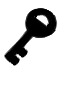
\includegraphics[scale=0.35]{\filepath/key}
\end{minipage}
\begin{minipage}[t]{6in}%6.25
#1
\end{minipage}
};
\end{tikzpicture}\\%
}}


\newcommand{\wrbox}[1]{{
\noindent
\centering
\begin{tikzpicture}
\node [wrbox] (box){
\begin{minipage}[c]{.2in}
%\hspace{-.2in}
%\dbend
{\Huge \bf !}
\end{minipage}
\begin{minipage}[t]{6in}%6.25
#1
\end{minipage}
};
\end{tikzpicture}\\%
}}
\newcommand{\hintbox}[1]{{
\noindent
\centering
\begin{tikzpicture}
\node [hnbox] (box){
\begin{minipage}[l]{6in}
\textbf{Hint:} {#1}
\end{minipage}
};
\end{tikzpicture}\\%
}
}
%white box
\newcommand{\whbox}[1]{{
\noindent
\centering
\begin{tikzpicture}
\node [hnbox] (box){
\begin{minipage}[l]{6in}
{#1}
\end{minipage}
};
\end{tikzpicture}\\%
}
}
%6.68
%END DEFINING BOX COMMANDS
%%%%%%%%%%%%%%%%%%%%%%%%%%%%%%%%%%%%%%%%%%%%%%%%%

%Box commands
%\thbox{...} makes a theorem box
%\thmbox{...} makes a theorem box labeled "Theorem"
%\prbox{...} makes a problem box
%\prbbox{...} makes a problem box labeled "Problem"
%\cpbox{...} makes a concept box labeled "Concept"
%\wrbox{...} makes a warning box.
%\dfbox{...} makes a definition box (same as problem box) labeled "> Definition"
%\sprbbox{...} makes a problem box labeled "Problem" (use this when you're making a copy of a previous problem box to put the solution afterwards; it has a numbering system separate from problems).

 
% for testing purposes only
\usepackage[english]{babel} 
\usepackage{blindtext} 
%%%%%%%%
%begin doc
%%%%%%%%
%%%%%%%%%%%%%%%%%%%%%%%%%%%%%%%%%%%%%%%%%%%%%%%%%
%DEFINING THE BOXES.
% Problem box (simple box, blue)
\tikzstyle{prbox} = [draw=black, fill=blue!20, very thick,
    rectangle, inner sep=10pt, inner ysep=10pt]
% Theorem box (double border, gray)
\tikzstyle{thbox} = [draw=black,double, fill=blue!10, very thick,
    rectangle, inner sep=10pt, inner ysep=10pt]
%\tikzstyle{fancytitle} =[fill=red, text=white]
% Concept box (shadowed, light green)
\tikzstyle{cpbox} = [drop shadow={
    shadow scale=1}, draw=black, fill=green!10, very thick,
    rectangle, inner sep=10pt, inner ysep=10pt]
\tikzstyle{wrbox} = [drop shadow={
    shadow scale=1}, draw=black, fill=yellow!10, very thick,
    rectangle, inner sep=10pt, inner ysep=10pt]
\tikzstyle{hnbox} = [draw=black, fill=white, very thick,
    rectangle, inner sep=10pt, inner ysep=10pt]
%END DEFINING BOXES
%%%%%%%%%%%%%%%%%%%%%%%%%%%%%%%%%%%%%%%%%%%%%%%%%
